\documentclass[14pt]{beamer}
%\usetheme{Singapore} %Gray with fade at top
%\useoutertheme[subsection=false]{miniframes} %Supppress subsection in header
\useinnertheme{rectangles} %Itemize/Enumerate boxes
\usecolortheme{seagull} %Color theme
\usecolortheme{rose} %Inner color theme

\definecolor{light-gray}{gray}{0.75}
\definecolor{dark-gray}{gray}{0.55}
\setbeamercolor{item}{fg=light-gray}
\setbeamercolor{enumerate item}{fg=dark-gray}

\setbeamertemplate{navigation symbols}{}
%\setbeamertemplate{mini frames}[default]
%\setbeamercovered{dynamics}
\setbeamerfont*{title}{size=\Large,series=\bfseries}
\setbeamerfont*{author}{size=\normalsize,series=\bfseries}
\setbeamerfont*{institute}{size=\normalsize}

\setbeamertemplate{frametitle}{\vspace{.5em}\bfseries\insertframetitle}
\newcommand{\heading}[1]{\noindent \textbf{#1}\\ \vspace{1em}}

\newcommand{\bigslide}[1]{
\bgroup
\setbeamercolor{background canvas}{bg=black!80!blue}
\frame{\vspace{4em}\Huge\textbf{\textcolor{white}{#1}}}
\egroup
}

\newcommand\Wider[2][3em]{%
\makebox[\linewidth][c]{%
  \begin{minipage}{\dimexpr\textwidth+#1\relax}
  \raggedright#2
  \end{minipage}%
  }%
}

\pagecolor{black}
\usepackage{pdfpages}

\usepackage{tikz}
\usetikzlibrary{shapes,arrows}

\usepackage{adjustbox}
\usepackage{alltt}
\usepackage{bbding}
\usepackage{color}
\usepackage{graphicx}
\usepackage{verbatim}
\usepackage{pbox}
\usepackage{amssymb}
\usepackage[english]{babel}
\usepackage[latin1]{inputenc}
\usepackage[T1]{fontenc}
\usepackage{lmodern}
\usepackage{listings}
\usepackage{ulem} % strikeout text

%\setbeamerfont{title}{size=\Huge,series=\bfseries}
\title{\textcolor{black}{The CloudyR Project:\\Statistical Cloud Computing in R with Amazon and Google}}

\author[]{\textcolor{black}{Thomas J. Leeper}}
\institute[]{
  \textcolor{black}{{\small London School of Economics and Political Science\\ \vspace{1em}
  Twitter: {\bfseries \href{http://www.twitter.com/thosjleeper}{@thosjleeper} \href{http://www.twitter.com/cloudyrproject}{@cloudyrproject}} \\
  GitHub: {\bfseries \href{http://www.github.com/leeper}{@leeper} \href{http://www.github.com/cloudyr}{@cloudyr} }\\
  {\bfseries \href{mailto:thosjleeper@gmail.com}{thosjleeper@gmail.com}}}}
}

\date[]{}

\begin{document}


\frame{\titlepage}

\section{Motivation}
\frame{\tableofcontents}
\frame{\tableofcontents[currentsection]}


\frame{
\begin{center}
\Large
This talk is about cloud computing.\\

\vspace{1em}

What is that?
\end{center}
}

% big data joke
\bgroup
\setbeamercolor{background canvas}{bg=black!80!blue}
\frame{
\Large
\visible<2>{\textcolor{red}{Cloud computing}}
\vspace{-0.5em}
\begin{center}
\textit{\textcolor{white}{
\only<1>{Big data}\only<2>{\sout{Big data}} is like teenage sex: everyone talks about it, nobody really knows how to do it, everyone thinks everyone else is doing it, so everyone claims they are doing it\dots}}\\

\vspace{1em}

\raggedleft \textcolor{white}{-- Dan Ariely, 2013}
\end{center}
}
\egroup


\frame{
\begin{center}
\includegraphics[width=.9\textwidth]{images/cloudcomputing.png}
\end{center}
}


\frame{

\frametitle{Cloud Computing 101}

Cloud computing refers to a variety of ideas:\\

\vspace{1em}

\begin{itemize}\itemsep1em
\item Software-as-a-Service (SaaS)
\item Platform-as-a-Service (PaaS)
\item Infrastructure-as-a-Service (IaaS)
\end{itemize}

\vspace{1em}

All of these shift computational tasks from a local machine to a server.

}

\frame{

\frametitle{Who are the major players?}

\begin{center}
\includegraphics[width=\textwidth]{images/cloud-market-share.png}
\end{center}

}


\frame{
\frametitle{Why cloud computing?}
\begin{itemize}\itemsep0.5em
\item<2-> Storage
\item<3-> Memory
\item<4-> Explicit parallelism
\item<5-> Security/Collaboration
\item<6-> Reproducibility
\item<7-> Data pipelines
\item<8-> SaaS
\end{itemize}
}


\begin{frame}
    \frametitle{Why cloud computing?}
    \begin{columns}[t]
        \begin{column}{.35\linewidth}
            \textbf{This Laptop}
            \begin{itemize}
            \item Intel Core i7 (4 cores)
            \item 8 GB memory
            \item 100 GB of usable storage
            \end{itemize}
        \end{column}
        \begin{column}{.65\linewidth}
			\textbf{What you can get on AWS}
        	\begin{itemize}
        	\item Equivalent AWS instance costs \$0.0928/hour
        	\item 96 cores and 384 GB memory costs \$4.608/hour
        	\item In theory unlimited number of instances
        	\item Storage is basically unlimited
        		\begin{itemize}
        		\item S3: \$0.023/GB-month
        		\item EBS: \$0.10/GB-month
        		\end{itemize}
        	\end{itemize}
        \end{column}
    \end{columns}
\end{frame}


\frame{

\frametitle{Simplest Use Case:\\Execute Code in the Cloud}

\begin{enumerate}\itemsep1em
\item Reserve an ``instance'' in the cloud
\item Fire up your favorite statistical software
\item Execute code as if you were running locally
\item Retrieve results
\end{enumerate}

}

% What does this mean for statisticians?
\bgroup
\setbeamercolor{background canvas}{bg=black}
\frame<1>[label=why]{
\large
\begin{center}
\textbf{\textcolor{white}{Why aren't researchers using cloud computing resources?}}

\vspace{2em}

\onslide<2->{\textcolor{white}{Statisticians and scientists may not know anything about how to set up high-performance computing infrastructure!}}

\vspace{2em}

\onslide<3->{\textcolor{white}{\textbf{I am one of those people!}}}
\end{center}
}

\frame{
\begin{quote}
\textcolor{white}{I started using SPSS in 1979, while studying cognitive psychology at the Leiden University. In these days I had to program SPSS-syntax on punched cards. The worst thing was not this card-interface, but it was the IBM job control language you had to include: total gibberish language that was needed to make your SPSS-job run on a mainframe somewhere in one of the university buildings.}
\end{quote}

\vspace{1em}
\textcolor{white}{{\footnotesize Source: Gerard van Meurs, \url{https://50-years-spss.com/user-stories/}}}
}

\againframe<1-3>{why}

\egroup




% cloudyr project scope
\begin{frame}
    \frametitle{The CloudyR Project}
    \begin{columns}
        \begin{column}{.5\linewidth}
          \includegraphics[width=\textwidth]{images/cloudyr_logo.png}
        \end{column}
        \begin{column}{.5\linewidth}
            \begin{itemize}\itemsep1em
            \item<2-> Make R Cloudier!
            
            \item<3-> Build easy-to-use, dependency-free software tools for working with any cloud service from R
            \end{itemize}
        \end{column}
    \end{columns}

\vspace{2em}

\onslide<4->{Eventual goal: \texttt{eval\_cloud("script.R")}}
\end{frame}

% cloudyr project strucutre
\begin{frame}
\frametitle{The CloudyR Project}
\begin{itemize}\itemsep1em
\item 100\% volunteer effort
\item We receive no funding from any cloud service
\item We build free and open source tools
\item Many contributors!
	\begin{itemize}
	\item Main AWS developer: Thomas Leeper
	\item Main GCS developer: Mark Edmondson
	\item Lots of PRs, bug reports, and documentation fixes from many, many people
	\end{itemize}
\end{itemize}
\end{frame}

\frame{
\frametitle{Why bother?}

Cloud providers have broad language support:\\

\vspace{1em}

\begin{itemize}\itemsep1em
\item AWS SDKs: Java .Net Node.js PHP Python Ruby Go (C++)
\item GCS SDKs: Java .Net Node.js PHP Python Ruby Go (C++)

\vspace{2em}

\onslide<2->{\Large\raggedleft \textbf{But where's R?}}
\end{itemize}
}

\frame{
\frametitle{R is a first-class statistics and data science language!}

\begin{center}
\includegraphics[width=\textwidth]{images/tiobe.png}
\end{center}
}



\frame{

\frametitle{Building R packages for cloud computing is difficult}

\begin{itemize}\itemsep1em
\item<2-> Wrap an existing SDK
	\begin{itemize}
	\item \url{https://github.com/hrbrmstr/roto.s3} (Requires Python \includegraphics[width=1em]{images/neutral-emoji.png})
	\item \url{https://cran.r-project.org/package=AWR} (Requires Java \includegraphics[width=1em]{images/vomit-emoji.png})
	\end{itemize}

\item<3-> Wrap the AWS Command Line Tools
	\begin{itemize}
	\item \href{https://github.com/cran/AWS.tools}{AWS.tools}, \href{https://github.com/lalas/awsConnect/}{awsConnect}
	\item Requires a system dependency \includegraphics[width=1em]{images/frowning-emoji.png}
	\item Very difficult to maintain \includegraphics[width=1em]{images/frowning-emoji.png}
	\end{itemize}

\item<4-> Build native R packages using web APIs \includegraphics[width=1em]{images/grinning-emoji.png}
\end{itemize}

}

\frame{
\begin{center}
\includegraphics[height=\textheight]{images/aws-services.png}
\end{center}
}


\frame{

\frametitle{Simplest Use Case}

End goal: \texttt{eval\_cloud("script.R")}

\vspace{1em}

What do we need in order to make that happen?\\

\vspace{1em}

\begin{itemize}
\item<2-> Low-level web API (HTTP) handling \onslide<3->{\checkmark}
\item<4-> Cloud storage infrastructure (S3) \onslide<5->{\checkmark}
\item<6-> User account management (IAM) \onslide<7->{\checkmark}
\item<8-> Cloud computing tools (EC2) \onslide<9->{\checkmark}
\item<10-> Secure shell connections\only<10->{\footnote{\url{https://github.com/ropensci/ssh}}} \onslide<11->{\checkmark}
\item<12-> High-level abstractions over the above
\end{itemize}

}


\frame{}
\section{Use Cases}
\frame{\tableofcontents[currentsection]}

\begin{frame}[fragile]\small
\begin{verbatim}
# 1. create an AWS account

# 2. load credentials into R
Sys.setenv("AWS_ACCESS_KEY_ID" = "my_key")
Sys.setenv("AWS_SECRET_ACCESS_KEY" = "my_secret")
Sys.setenv("AWS_DEFAULT_REGION" = "us-east-1")
\end{verbatim}
\end{frame}


% storage: aws.s3
\bigslide{Storage}

\begin{frame}[fragile]\small
\begin{verbatim}
# cloud storage
library("aws.s3")

# put an R object into the cloud
s3saveRDS(mtcars, "s3://bucket/mtcars.rds")

# get an R object from the cloud
s3readRDS("s3://bucket/mtcars.rds")
\end{verbatim}
\end{frame}

\begin{frame}[fragile]\small
\begin{verbatim}
# manipulate buckets
put_bucket()
get_bucket()
delete_bucket()

# manipulate objects
put_object()
get_object()
delete_object()
\end{verbatim}
\end{frame}

\begin{frame}[fragile]\small
\begin{verbatim}
# higher-level functions
s3source()

s3save()
s3load()

s3read_using()
s3write_using()

# streaming R connection (rb)
s3connection()
\end{verbatim}
\end{frame}

% notifications: aws.sns
\bigslide{Notifications}

\begin{frame}[fragile]
\begin{verbatim}
# notifications
library("aws.sns")

# create a "topic"
topic <- create_topic(name = "jsm-example")

# subscribe to it
subscribe(topic, "me@example.com", "email")
subscribe(topic, "1-111-555-1234", "sms")
\end{verbatim}
\end{frame}

\begin{frame}[fragile]
\begin{verbatim}
# R script
done <- FALSE
while (!done) {
  # long-running thing
  done <- TRUE
}

# send notification
publish(
  topic = topic,
  message = "Your script is done. -R",
  subject = "Done!"
)
\end{verbatim}
\end{frame}



% compute
\bigslide{Computing}

	% aws.aec2
	% clusters (coming soon!)
	% aws.iam: access to compute and storage resources
\begin{frame}[fragile]\small
\begin{verbatim}
library("aws.ec2") # cloudyr/aws.ec2

# RStudio-configured EC2 image
# http://www.louisaslett.com/RStudio_AMI/
image <- "ami-fd2ffe87"

# create keypair
my_keypair <- create_keypair("jsm-keys")
cat(my_keypair$keyMaterial, file = "my.pem")

my_sg <- create_sgroup(
  "jsm-sg",
  "Allow my IP",
  vpc = describe_vpcs()[[1]]
)
authorize_ingress(my_sg)
\end{verbatim}
\end{frame}

\begin{frame}[fragile]\small
\begin{verbatim}
# fire up instance
i <- run_instances(
  image = image, type = "t2.micro",
  sgroup = my_sg,
  subnet = "subnet-b815a6e0",
  keypair = my_keypair
)

ip <- allocate_ip("vpc")
associate_ip(i, ip)

browseURL(paste0("http://", ip$publicIp))
\end{verbatim}
\end{frame}


\begin{frame}[fragile]\small
\begin{verbatim}
# log in to instance
library("ssh")
session <- ssh::ssh_connect(
  paste0("ubuntu@", ip$publicIp),
  keyfile = "my.pem",
  passwd = "rstudio"
)

# hello world!
cat("'hello world!'\n", file = "helloworld.R")
# upload it to instance
ssh::scp_upload(session, "helloworld.R")

# execute script on instance
ssh::ssh_exec_wait(session, "Rscript helloworld.R")

# disconnect from instance
ssh_disconnect(session)
\end{verbatim}
\end{frame}


\begin{frame}[fragile]\small
\begin{verbatim}
# cleanup
stop_instances(i[[1]])
terminate_instances(i[[1]])

release_ip(ip)

revoke_ingress(my_sg)

delete_sgroup(sgroup = my_sg)
delete_keypair(my_keypair)
\end{verbatim}
\end{frame}

\frame{

\frametitle{A couple useful packages}

\url{https://cran.r-project.org/package=ssh}

\vspace{1em}

\url{https://github.com/cloudyr/rmote}

\vspace{1em}

\url{https://cran.r-project.org/package=remoter}

}


% software as a service
\bigslide{SaaS}

% aws.polly
% aws.translate
% aws.transcribe
\begin{frame}[fragile]\small
\begin{verbatim}
library("aws.polly")

msg_en <- "Thanks for attending the Cloud and Distributed Computing for Statisticians presentation at JSM 2018. You've been a great audience!"

vec_en <- synthesize(msg_en, voice = "Joanna")

tuneR::play(vec_en)
\end{verbatim}
\end{frame}

\begin{frame}[fragile]\small
\begin{verbatim}
library("aws.translate")

msg_es <- translate(msg_en, from = "en", to = "es")
vec_es <- synthesize(msg_es, voice = "Penelope")
tuneR::play(vec_es)

msg_ru <- translate(msg_en, from = "en", to = "ru")
vec_ru <- synthesize(msg_ru, voice = "Maxim")
tuneR::play(vec_ru)
\end{verbatim}
\end{frame}

\begin{frame}[fragile]\small
\begin{verbatim}
library("aws.comprehend")

detect_language(msg_en)
detect_language(msg_es)
detect_language(msg_ru)

\end{verbatim}
\end{frame}


\begin{frame}[fragile]\small
\begin{verbatim}
library("aws.transcribe")

tuneR::writeWave(vec_en, "english.wav")
aws.s3::put_object(
 "english.wav",
 "s3://jsm2018cloudyrexample/english.wav",
 acl = "public-read"
)

start_transcription(
 "jsm2018-example",
 paste0("https://s3.amazonaws.com/",
        "jsm2018cloudyrexample/",
        "english.wav")
)

tr <- get_transcription("jsm2018")$Transcriptions
cat(strwrap(tr, 60), sep = "\n")
\end{verbatim}
\end{frame}





% crowdsourcing
\bigslide{Crowdsourcing}

\begin{frame}[fragile]
\large
\begin{center}
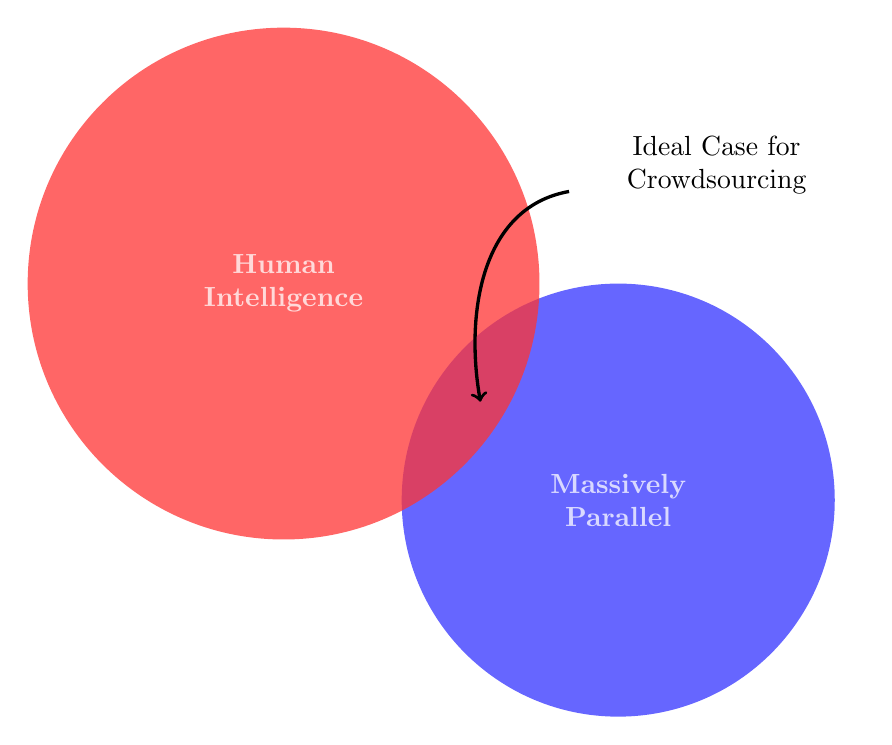
\begin{tikzpicture}
    \fill[blue!80,opacity=0.75] (4.25,0.25) circle (2.75cm) 
        node[text=white, align=center, text width=3cm] {\textbf{Massively\\ Parallel}};
    \fill[red!80,opacity=0.75] (0,3) circle (3.25cm) 
        node[text=white, align=center, text width=3cm] {\textbf{Human\\ Intelligence}};
    \node[align=center, text width=3.5cm] at (5.5,4.5) (c) {Ideal Case for\\ Crowdsourcing};
    \draw[->,very thick] (c) to [out = 190, in = 100, looseness = 1] (2.5,1.5);
% use-cases: scraping, coding, human subjects research
% crowdsourcing is a form of parallel computing
\end{tikzpicture}
\end{center}
\end{frame}


% PLACEHOLDER
\bgroup
\begin{frame}[fragile]
% Define block styles
\tikzstyle{decision} = [diamond, draw, fill=blue!20, 
    text width=4.5em, text badly centered, node distance=3cm, inner sep=0pt]
\tikzstyle{block} = [rectangle, draw, fill=blue!20, draw=none,
    text width=2cm, text centered, rounded corners, minimum height=4em]
\tikzstyle{line} = [draw, -latex', line width=1.5pt, color=gray!95]
\tikzstyle{cloud} = [draw, ellipse,fill=blue!20, draw=none, minimum height=2em]

\begin{adjustbox}{max totalsize={\textwidth}{\textheight},center}
\begin{tikzpicture}[scale=0.5,node distance = 2cm, auto]
    % Place nodes
    \node [block, text=white, fill=blue!65, minimum width=3cm, text width=4cm] (init) {\Large\textbf{Data Need}};
    \node [block, below of=init, node distance=5cm, minimum width=3cm, text width=5cm, fill=gray!15] (design) {\Large\textbf{Design Data Entry Form}};
%    	Register HITType
%    	};
    \node [block, below of=design, node distance=5cm, minimum width=4cm, text width=4cm] (createhit) {
    	\Large \textbf{Create HIT(s)}
    	};
    \node [cloud, right of=createhit, node distance=6cm, fill=red!20] (assignment3) {Assignment};
    \node [cloud, above of=assignment3, node distance=1cm, fill=red!20] (assignment2) {Assignment};
    \node [cloud, above of=assignment2, node distance=1cm, fill=red!20] (assignment1) {Assignment};
    \node [cloud, below of=assignment3, node distance=1cm, fill=red!20] (assignment4) {Assignment};
    \node [cloud, below of=assignment4, node distance=1cm, fill=red!20] (assignment5) {Assignment};
    \node [block, right of=assignment3, node distance=6cm, minimum width=3cm, text width=3cm] (review) {\Large \textbf{Review}};
    \node [block, above of=review, node distance=10cm, text=white, fill=blue!65, minimum width=3cm, text width=4cm] (analyze) {\Large\textbf{Analyze data}};
    
    \node [left of=init, node distance=6cm, align=left] (R) {\Large\textbf{R}};
    \node [below of=R, node distance=5cm, align=left] (html) {\Large\textbf{HTML}};
    \node [below of=html, node distance=5cm, align=left] {\Large\textbf{MTurk}};
    
    %     % Draw edges
    \path [line] (init) -- (design);
    \draw [line] (design) to [out=270,in=90] (createhit);
    \draw [line] (createhit) to [out=20, in=180] (assignment1);
    \draw [line] (createhit) to [out=10, in=180] (assignment2);
    \draw [line] (createhit) to [out=0, in=180] (assignment3);
    \draw [line] (createhit) to [out=350, in=180] (assignment4);
    \draw [line] (createhit) to [out=340, in=180] (assignment5);
    \draw [line] (assignment1) to [out=0, in=160] (review);
    \draw [line] (assignment2) to [out=0, in=170] (review);
    \draw [line] (assignment3) to [out=0, in=180] (review);
    \draw [line] (assignment4) to [out=0, in=190] (review);
    \draw [line] (assignment5) to [out=0, in=200] (review);
    \path [line] (review) -- (analyze);
\end{tikzpicture}
\end{adjustbox}
\end{frame}
\egroup

\bgroup
\setbeamercolor{background canvas}{bg=black}
\begin{frame}
\Wider[1em]{\vspace{1em}
{\color{white}\texttt{a = GenerateHTMLQuestion(file = "hit.html")\\
\vspace{1em}
hit = CreateHIT(\\
\hspace{0.5em}  title = "Short Survey",\\
\hspace{0.5em}  description = "5 question survey",\\
\hspace{0.5em}  keywords = "survey, questionnaire",\\
\hspace{0.5em}  duration = seconds(hours = 1)\\
\hspace{0.5em}  reward = .10,\\
\vspace{1em}
\hspace{0.5em}  assignments = 5000,\\
\hspace{0.5em}  expiration = seconds(days = 4),\\
\hspace{0.5em}  question = a\$string,\\
)
}}}
\end{frame}
\egroup


\begin{frame}[fragile]
\frametitle{Anatomy of an MTurkR App}
% Define block styles
\begin{center}
    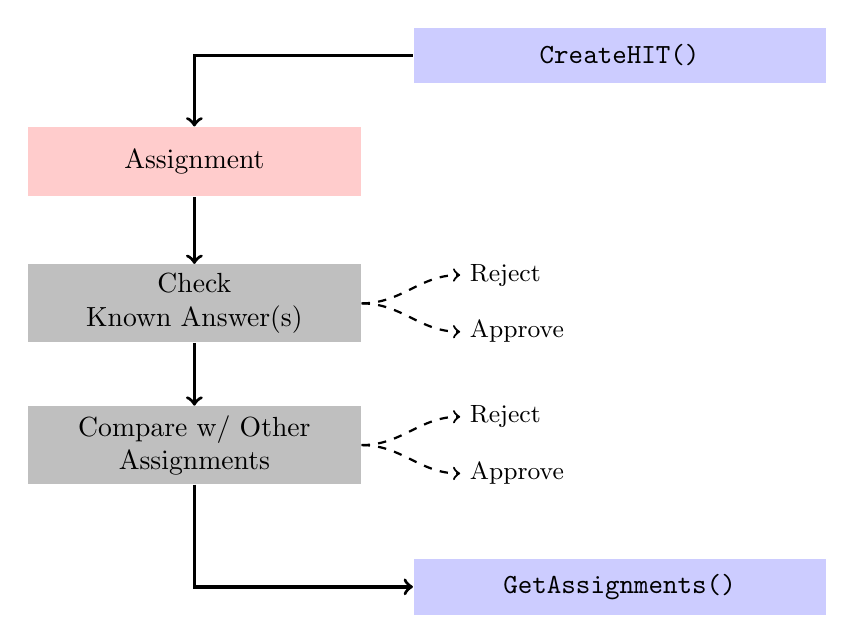
\begin{tikzpicture}[scale=0.9]
    \node[fill=red!20, text width=4cm, minimum height=2.5em, align=center] at (0,6) (assign) {Assignment};
    \node[fill=blue!20, text width=5cm, minimum height=2em, align=center] at (6,7.5) (create) {\texttt{CreateHIT()}};
    \draw[->, very thick] (create) -| (assign);
    \node[fill=gray!50, text width=4cm, align=center] at (0,4) (known) {Check\\ Known Answer(s)};
    \draw[->, very thick] (assign) to (known);
    \node [text width = 2cm] at (5,4.4) (reject1) {\small Reject};
    \node [text width = 2cm] at (5,3.6) (approve1) {\small Approve};
    \draw[->, dashed, thick] (known) to [out=0, in=180] (approve1);
    \draw[->, dashed, thick] (known) to [out=0, in=180] (reject1);
    \node[fill=gray!50, text width=4cm, align=center] at (0,2) (hit) {Compare w/ Other Assignments};
    \draw[->, very thick] (known) to (hit);
    \node [text width = 2cm] at (5,2.4) (reject2) {\small Reject};
    \node [text width = 2cm] at (5,1.6) (approve2) {\small Approve};
    \draw[->, dashed, thick] (hit) to [out=0, in=180] (approve2);
    \draw[->, dashed, thick] (hit) to [out=0, in=180] (reject2);
    \node[fill=blue!20, text width=5cm, minimum height=2em, align=center] at (6,0) (results) {\texttt{GetAssignments()}};
    \draw[->, very thick] (hit) |- (results);
    \end{tikzpicture}
\end{center}
\end{frame}

\bgroup
\setbeamercolor{background canvas}{bg=black}
\begin{frame}
\small
\begin{alltt}
\textcolor{white}{BulkCreateFromURLs(}\\
\textcolor{white}{\hspace{0.5em}  url = paste0("https://example.com/",1:10,".html"),}\\

\textcolor{white}{\hspace{0.5em}  title = "Image Categorization",}\\
\textcolor{white}{\hspace{0.5em}  description = "Describe contents of an image",}\\
\textcolor{white}{\hspace{0.5em}  keywords = "categorization, image",}\\
\textcolor{white}{\hspace{0.5em}  reward = .01,}\\
\textcolor{white}{\hspace{0.5em}  duration = seconds(minutes = 5),}\\

\textcolor{white}{\hspace{0.5em}  annotation = "My Project",}\\
\textcolor{white}{\hspace{0.5em}  expiration = seconds(days = 4),}\\
\textcolor{white}{\hspace{0.5em}  auto.approval.delay = seconds(days = 1)}\\
\textcolor{white}{)}
\end{alltt}
\end{frame}
\egroup


\begin{frame}[fragile]
\textbf{Get back a data.frame:}\\
\vspace{1em}
\texttt{GetAssignments(annotation = "My Project")}\\
\vspace{1em}
\def\arraystretch{1.5}

\textbf{Example:}
\begin{tabular}{rl}
An image coding task with & \textbf{27,500 images}\\
                      took & \textbf{225 workers}\\
                     about & \textbf{75 minutes}\\
                  and cost & \textbf{\$412.50}\\
\end{tabular}

\vspace{1em}
{\small \textcolor{gray}{\textbf{Pay workers with:}\\ \texttt{ApproveAssignments(annotation = "My Project")}}}
\end{frame}



\frame{}
\section{Conclusion}
\frame{\tableofcontents[currentsection]}


\frame{
\frametitle{CloudyR isn't just AWS}
\begin{itemize}\itemsep1em
\item GCS APIs are much cleaner
\item Storage: googleCloudStorageR
\item Compute: googleComputeEngineR
\item Others: gcloudR (client for \textit{any} GCS API)

\vspace{1em}

\item<2-> In the pipeline:\\ Meta packages to abstract across cloud services
\end{itemize}
}

\frame{
\frametitle{What's next for CloudyR?}
\begin{itemize}\itemsep1em
\item Databases\\ (DynamoDB, Redshift, RDS)
\item Machine Learning as a Service\\ (AWS Glue, ML, SageMaker)
\item Everything!?
\end{itemize}
}

\begin{frame}
    \frametitle{We can always use volunteers!}
    
    \begin{columns}[t]
        \begin{column}{.52\linewidth}
          \textbf{Experienced Developers}\\
          \begin{itemize}\itemsep1em
          \item Build packages for new cloud services
          \item Expand our scope beyond AWS and GCS
          \item Contribute PRs
          \end{itemize}
        \end{column}
        \begin{column}{.48\linewidth}
			\textbf{Beginner Developers}\\
			\begin{itemize}\itemsep1em
			\item Feature requests
			\item Improve our documentation and examples
			\item Improve our tests
			\item Use packages and find bugs
			\end{itemize}
        \end{column}
    \end{columns}
\end{frame}





\bgroup
\setbeamercolor{background canvas}{bg=black}
\begin{frame}
    \vspace{1em}
    {\color{white}\texttt{\noindent \# Start Cloud Computing\\
    \vspace{1.5em}
    install\_github("cloudyr/awspack")\\
    install\_github("cloudyr/gcloudR")\\
    \vspace{1.5em}
    \# Questions?\\
    \# \href{https://twitter.com/thosjleeper}{Twitter @thosjleeper} \href{https://twitter.com/cloudyrproject}{@cloudyrproject}\\
    \# \url{https://github.com/cloudyr}\\
    \# \url{http://cloudyr.github.io}\\
    \# \href{mailto:thosjleeper@gmail.com}{thosjleeper@gmail.com}
    }}
\end{frame}
\egroup


\bgroup
\setbeamercolor{background canvas}{bg=black}
\frame{}
\egroup

\end{document}
